\documentclass[1pt]{article}
\usepackage[UTF8]{ctex}

\usepackage{amsmath, amsthm, amssymb, bm, graphicx, hyperref, mathrsfs}
\title{{\Huge{\textbf{基础物理实验——实验报告}}}\\测量介质中的声速}
\author{赵雅鹏\qquad2100011762\\化学与分子工程学院}
\date{\today}
\linespread{1.5}
\usepackage{geometry}
\geometry{a4paper,left=0.9cm,right=0.9cm,top=1.5cm,bottom=1.3cm}
\newtheorem{theorem}{定理}[section]
\newtheorem{definition}[theorem]{定义}
\newtheorem{lemma}[theorem]{引理}
\newtheorem{corollary}[theorem]{推论}
\newtheorem{example}[theorem]{例}
\newtheorem{proposition}[theorem]{命题}
\usepackage[small]{titlesec}
\usepackage{makecell}


\begin{document}

  \begin{titlepage}
    \vspace*{\fill}
    \begin{center}
      {\Huge{\textbf{基础物理实验}}}\\[0.5cm]
		{\Huge{\textbf{——测量介质中的声速实验报告}}}\\[0.5cm]
      {\Large{赵雅鹏\qquad2100011762}}\\[0.4cm]
      {\Large{化学与分子工程学院}}\\[0.3cm]
      {\Large{\today}}
    \end{center}
    \vspace*{\fill}
  \end{titlepage}

\pagenumbering{roman}
\setcounter{page}{1}
\newpage
\pagenumbering{Roman}
\setcounter{page}{1}
\setcounter{page}{1}
\pagenumbering{arabic}



\section{共振频率的测量结果}
\centerline{$f_0$ = 40.000kHz}
\section{极值法}
	\begin{center}
	\begin{tabular}{|c|c|c|c|c|c|c|c|c|c|c|}
	\hline
	测量序数&1&2&3&4&5&6&7&8&9&10\\
	\hline
	正向测量距离/mm&44.062&48.432&52.942&57.462&62.732&66.091&70.419&74.739&79.088&83.349\\
	\hline
	正向测量峰-峰值电压/V&7.76&7.12&6.32&5.28&4.88&4.16&3.70&3.88&3.84&3.84\\
	\hline
	反向测量距离/mm&96.125&91.808&87.700&82.979&79.513&74.141&69.958&66.461&61.310&56.940\\
	\hline
	反向测量峰-峰值电压/V&3.20&3.44&3.52&3.76&3.84&3.84&4.00&3.92&4.72&5.04\\
	\hline
	\end{tabular}
	\end{center}
%逐差法处理数据,给出声速测量结果,评价不确定度
逐差法计算(由于没有告知示波器允差,故在此忽略示波器允差,实际上使用的示波器精度非常高,估计测量距离的仪器和螺旋测微器允差类似,实际上也足够小可以忽略,故次估算合理)\\
正向测量:\qquad$\dfrac{\lambda}{2}=\dfrac{(x_{10}+x_9+x_8+x_7+x_6)-(x_5+x_4+x_3+x_2+x_1)}{5^2}=4.322$mm ;\qquad $v=\dfrac{\lambda}{2}\times2f_0=345.8$m/s\\
\centerline{随机误差: $\sigma_{\lambda} = \dfrac{s}{\sqrt n}=\sqrt{\dfrac{1}{n(n-1)}[\sum_{i=0}^{5}(\delta_i-\bar{\delta})^2]}=0.041$mm(PS:$\delta_i=x_{i+5}+x_i,\bar{\delta}=\sum_{i=0}^{5}\delta_i)$}\\
\centerline{系统误差:$e_1=0.004$mm}\\
\centerline{$\therefore \sigma_\lambda = \sqrt{(\sigma_{\lambda})^2+e_1^2}=0.041$mm$\Rightarrow \lambda = 4.32$mm\qquad 相对不确定度=$\dfrac{0.041}{4.32}=0.9\%$}\\
\centerline{$\therefore \sigma_v = v \dfrac{\sigma_\lambda}{\lambda} =3.3 $m$\cdot s^{-1} $}\\
\centerline{$v=\lambda\cdot f = 346 $m/s}\\
反向测量:\qquad$\dfrac{\lambda}{2}=\dfrac{(x_5+x_4+x_3+x_2+x_1)-(x_{10}+x_9+x_8+x_7+x_6)}{5^2}=4.373$mm ;\qquad $v=\dfrac{\lambda}{2}\times2f_0=$349.8m/s\\
\centerline{随机误差: $\sigma_{\lambda} = \dfrac{s}{\sqrt n}=\sqrt{\dfrac{1}{n(n-1)}[\sum_{i=0}^{5}(\delta_i-\bar{\delta})^2]}=0.034$mm(PS:$\delta_i=x_{i+5}+x_i,\bar{\delta}=\sum_{i=0}^{5}\delta_i)$}\\
\centerline{系统误差:$e_1=0.004$mm}\\
\centerline{$\therefore \sigma_\lambda = \sqrt{(\sigma_{\lambda})^2+e_1^2}=0.034$mm$\Rightarrow \lambda = 4.37$mm\qquad 相对不确定度=$\dfrac{0.037}{4.37}=0.8\%$}\\
\centerline{$\therefore \sigma_v = v \dfrac{\sigma_\lambda}{\lambda} =2.7 $m$\cdot s^{-1} $}\\
\centerline{$v=\lambda\cdot f = 350 $m/s}\\
\centerline{$\therefore v=\dfrac{345.8+349.8}{2}=348$(m/s)}




\section{相位法}
	\begin{center}
	\begin{tabular}{|c|c|c|c|c|c|c|c|c|c|c|}
	\hline
	测量序数$x$&1&2&3&4&5&6&7&8&9&10\\
	\hline
	正向测量距离y/mm&26.019&30.632&35.141&39.480&43.929&48.292&52.620&57.022&61.361&65.773\\
	\hline
	反向测量距离y/mm&74.100&69.668&65.348&61.220&56.790&52.531&48.128&43.710&39.308&34.913\\
	\hline
	\end{tabular}
	\end{center}
%最小二乘法处理数据,给出声速测量结果,评价不确定度
最小二乘法计算(由于没有告知示波器允差,故在计算不确定度时忽略示波器允差,实际上使用的示波器精度非常高,估计测量距离的仪器和螺旋测微器允差类似,实际上也足够小可以忽略,故次估算合理)\\
正向测量:\qquad $\bar{y}=\dfrac{\sum_{i=0}^{10}y_i}{10}=46.0269(mm)$;\qquad $\bar{x}=\dfrac{\sum_{i=0}^{10}x_i}{10}=5.5$\\
\centerline{$\overline{xy}=\dfrac{1}{10} \sum_{i=0}^{10} x_iy_i=289.4518
\qquad \bar{x^2}=\dfrac{1}{10} \sum_{i=0}^{10} x_i^2=38.5$}\\
\centerline{$\lambda = \dfrac{\overline{xy}-\bar{x}\bar{y}}{\overline{x^2}-(\bar{x})^2}=\dfrac{289.4518-46.0269\times5.5}{38.5-5.5^2}=4.400$(mm)}\\
\centerline{$v=\lambda f_0=352.0$m/s}\\
\centerline{$ r = \dfrac{\sum _{i=1}^{10}(x_{i} - \stackrel{-}{x})\cdot(y_{i} - \stackrel{-}{y})}{\sqrt{\sum _{i=1}^{10}(x_{i} - \stackrel{-}{x})^{2} \cdot \sum _{i=1}^{10}(y_{i} - \stackrel{-}{y})^{2}}} = 0.9999746$}\\
\centerline{随机误差: $\sigma_{\lambda} =  \lambda \sqrt{\dfrac{\frac{1}{r^{2}}-1}{n-2}}=0.011$mm}\\
\centerline{系统误差:$e_1=0.004$mm}\\
\centerline{$\therefore \sigma_\lambda = \sqrt{(\sigma_{\lambda})^2+e_1^2}=0.011$mm$\Rightarrow \lambda = 4.40$mm\qquad 相对不确定度=$\dfrac{0.011}{4.400}=0.3\%$}\\
\centerline{$\therefore \sigma_v = v \dfrac{\sigma_\lambda}{\lambda} =1.1 $m$\cdot s^{-1} $}\\
\centerline{$v=\lambda\cdot f = 352 $m/s}\\
反向测量:\qquad $\bar{y}=\dfrac{\sum_{i=0}^{10}y_i}{10}=54.5716(mm)$;\qquad $\bar{x}=\dfrac{\sum_{i=0}^{10}x_i}{10}=5.5$\\
\centerline{$\overline{xy}=\dfrac{1}{10} \sum_{i=0}^{10} x_iy_i=264.52974
\qquad \bar{x^2}=\dfrac{1}{10} \sum_{i=0}^{10} x_i^2=38.5$}\\
\centerline{$-\lambda = \dfrac{\overline{xy}-\bar{x}\bar{y}}{\overline{x^2}-(\bar{x})^2}=\dfrac{264.5274-55.5716\times5.5}{38.5-5.5^2}=-4.344$(mm)}\\
\centerline{$v=\lambda \cdot f_0=348$m/s}\\
\centerline{$ r = \dfrac{\sum _{i=1}^{10}(x_{i} - \stackrel{-}{x})\cdot(y_{i} - \stackrel{-}{y})}{\sqrt{\sum _{i=1}^{10}(x_{i} - \stackrel{-}{x})^{2} \cdot \sum _{i=1}^{10}(y_{i} - \stackrel{-}{y})^{2}}} = 0.999976$}\\
\centerline{随机误差: $\sigma_{\lambda} =  \lambda \sqrt{\dfrac{\frac{1}{r^{2}}-1}{n-2}}=0.011$mm}\\
\centerline{系统误差:$e_1=0.004$mm}\\
\centerline{$\therefore \sigma_\lambda = \sqrt{(\sigma_{\lambda})^2+e_1^2}=0.011$m$m\Rightarrow \lambda = 4.34$mm;\qquad 相对不确定度:$\dfrac{0.011}{4.34}=0.3\%$}\\
\centerline{$\therefore \sigma_v = v \dfrac{\sigma_\lambda}{\lambda} =1.1 $m$\cdot s^{-1} $}\\
\centerline{$v=\lambda\cdot f = 352 $m/s}\\
\centerline{$\therefore v=\dfrac{352.0+347.6}{2}=350$m/s}





\section{气体参量法}
	\begin{center}
	\begin{tabular}{|c|c|c|c|c|}
	\hline
	温度 $\theta$ &相对湿度&水的饱和蒸汽压 $p_s$ &水的分压$p_w$ & 大气压$p$ \\
	\hline
	$23.0^{\circ}$C&45&2809.1Pa&62.424&766.0mmHg\\
	\hline
	\end{tabular}\\
	\end{center}
	\qquad \qquad\qquad\qquad\qquad\qquad\qquad\qquad 声速($T_0=273.15^{\circ}$C):
	\begin{center}
	$v=331.45\times \sqrt{(1+\dfrac{\theta}{T_0})(1+\dfrac{0.3192p_w}{p})}=345$m/s
	\end{center}


\section{水中声速的测量(频率1.8000MHz)}
	\begin{center}
	\begin{tabular}{|c|c|c|c|c|c|c|c|c|c|c|}
	\hline
	测量序数&1&2&3&4&5&6&7&8&9&10\\
	\hline
	正向测量距离/cm&1.7842&1.8682&1.9517&2.0350&2.1172&2.1978&2.2856&2.3690&2.4520&2.5348\\
	\hline
	反向测量距离/cm&3.0262&2.9421&2.8591&2.7767&2.6955&2.6144&2.5315&2.4468&2.3638&2.2812\\
	\hline
	\end{tabular}
	\end{center}
逐差法计算\\
正向测量:\qquad$\dfrac{\lambda}{2}=\dfrac{(x_{10}+x_9+x_8+x_7+x_6)-(x_5+x_4+x_3+x_2+x_1)}{5^2}=0.08332$cm\\
 \centerline{$v=\dfrac{\lambda}{2}\times2f_0=1.500\times10^3$m/s}\\
反向测量:\qquad$\dfrac{\lambda}{2}=\dfrac{(x_5+x_4+x_3+x_2+x_1)-(x_{10}+x_9+x_8+x_7+x_6)}{5^2}=0.08248$cm\\
\centerline{$v=\dfrac{\lambda}{2}\times2f_0=1.485\times10^3$m/s}\\
\centerline{$\therefore v=\dfrac{1.500\times10^3+1.485\times10^3}{2}=1.492\times10^3$m/s}\\
\centerline{同理进行不确定度的计算后可知 $v=1.49\times 10^3$m/s}

\section{分析与讨论}
	\begin{figure}[htbp]
	\centering
	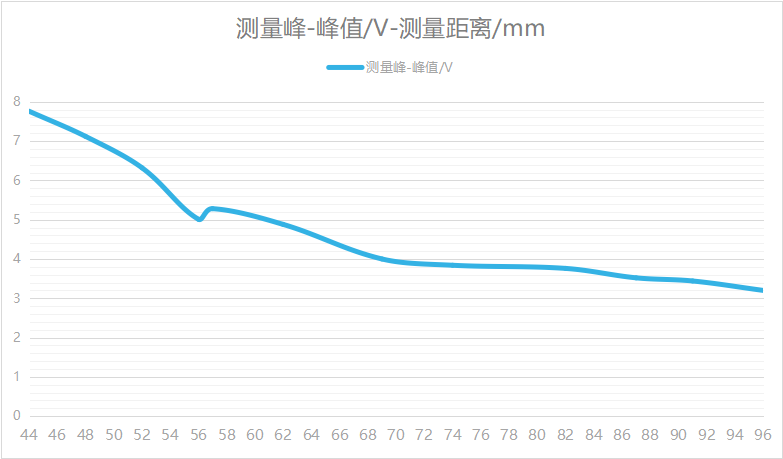
\includegraphics[scale=0.8]{diminishing.png}
	\caption{峰-峰值电压随距离衰减图}
\end{figure}
由图知,声波能量随传播距离衰减规律:峰-峰值电压随距离增大而衰减,且距离越大,衰减得越慢。




\section{收获与感想}
本次实验最大的感想就是,做物理实验除了做实验外,分析数据也很不容易,分析计算数据和计算不确定度,都是一项需要认真细致,有耐心的耗时工程。

本次实验发现,连接示波器、信号源以及测量仪器的数据线如果摆放很乱,会影响信号,导致示波器上面显示的信号不稳定,故需要摆放整齐。

以及使用\LaTeX 制作实验报告,可以将电脑带入实验室记录数据提升效率,既在实验记录本上记录数据,同时也计入\LaTeX 可以提升学习效率。

示波器上的正弦波和李萨如图形周期性变化,李萨如图形可以找到成为线形的情况,相比正弦波达到极值进行观察更容易,故相位法测量更为方便,精度更高。

\end{document}























+